\documentclass{subfiles}

\begin{document}
    \marginnote{\textit{\textbf{VL 12}}, 22.05.2023, 11:45}
    Das Verhalten von $t\mapsto \abs{\tau(t,x)}^2$ ist durch die folgende Grafik gezeigt.
    \begin{figure}[H]
        \centering
        \begin{tikzpicture}
            \draw[->] (-3, 0) -- (4.2, 0) node[right] {$x$};
            \draw[->] (0, -0.5) -- (0, 1) node[above] {$y$};
            \draw[scale=0.5, domain=0:6, smooth, variable=\t] plot ({\t},{1});
            \draw[scale=0.5, domain=0:6, smooth, variable=\t] plot ({\t},{1/(1+(1^2)/(4 * t * (1+t)) * sin((t*2)^(1/2)*1))});
        \end{tikzpicture}
    \end{figure}

    \subsection{Der harmonische Oszillator I}
    Der harmonische Oszillator ist ein Mechanik gut bekanntes schwingendes System, antreffbar beispielsweise in Form einer schwingenden Masse. Ihn zeichnet dabei durch das Vorverb \emph{harmonisch} angedeutete lineare Rückstellkraft $F = -k\cdot x$ aus, welche Resultat des Kraftpotentials $V = 1/2\cdot k\cdot x^2$ ist. Ein quantenmechanisches Pendant wären zwei gekoppelte, schwingende Moleküle, welche in der Festkörperphysik noch auf sogenannte \emph{Gitterschwindungen} bezüglich der Anzahl schwingender Moleküle verallgemeinert werden. Wir werden uns nun dem quantenmechanischen harmonischen Oszillator mithilfe der \emph{analytischen Methode} nach Sommerfeld nähern. Zu einem späteren Zeitpunkt werden wir uns ebenfalls mit dem \emph{algebraischen Ansatz} nach Dirac beschäftigen. Ausgangspunkt ist wieder die Eigenwertgleichung $H(\psi) = \lambda\cdot\psi$ mit dem Hamiltonoperator $H := P^2/(2m) + V(Q)$ mit $V:(k\cdot x^2/2)$ und $k\in\R$ als Kopplungskonstante. Daraus ergibt sich für einen Eigenwert $\lambda\in\sigma_P(H)$ wieder
    \[
        \Bbra{\dv{x}}^2\psi(x) = -\frac{2m}{\hbar^2}\cdot\Bbra{\lambda - \frac{k}{2}\cdot x^2}\cdot\psi(x).
    \]
    Im nächsten Schritt wollen wir die Lösung $\psi(x)$ transformieren zu einer einheitenlosen Funktion $u(x)$. Hierzu wählen wir die Transformation $\Phi:=\bigl(\sqrt{\omega\cdot m/\hbar}\cdot x\bigr)$, sodaß $\psi(x) = (u\circ \Phi)(x)$ gilt. Damit können wir die Differentialgleichung umformen zu
    \[
        \Bbra{\dv{x}}^2(u\circ\Phi)(x) = -\frac{2m}{\hbar^2}\cdot\Bbra{\lambda - \frac{k}{2}\cdot x^2}\cdot\psi(x)
    \]
    Mithilfe der Kettenregel folgern wir $d(u\circ\Phi)(x)(1) = du(\Phi(x))(1)\cdot d\Phi(x)(1)$, sodaß mit den Definitionen und zweifacher Ausführung gilt
    \[
        \Bbra{\dv{x}}^2(u\circ\Phi)(x) = \frac{\omega\cdot m}{\hbar}\cdot\Bbra{\dv{x}}^2(u\circ\Phi)(x).
    \]
    Damit können wir weiter ausformulieren:
    \[
        -\frac{\hbar^2}{2m}\cdot\frac{\omega\cdot m}{\hbar}\cdot\Bbra{\dv{x}}^2(u\circ\Phi)(x) = \lambda\cdot (u\circ\Phi)(x) - \cdot x^2\cdot(u\circ\Phi)(x).
    \]
    Mit der Definition $\eta := 2\cdot\lambda / (\hbar\cdot\omega)$ können wir die Energie $\lambda = \eta\cdot\hbar\cdot\omega/2$ ausdrücken und erhalten 
    \[
        -\frac{\hbar\cdot\omega}{2}\cdot\Bbra{\dv{x}}^2(u\circ\Phi)(x) = \frac{\hbar\cdot\omega}{2}\cdot\cdot\eta\cdot(u\circ\Phi)(x) - \frac{k}{2}\cdot x^2\cdot (u\circ\Phi)(x).
    \]
    \vspace{1cm}
    \[
        \Bbra{\dv{x}}^2(u\circ\Phi)(x) = (\eta - (u\circ\Phi)(x)^2)
    \]
    \[\Bbra{\dv{x}}(\psi\circ u^{-1})(x) + (\eta^{-1}(x) - u^{-1}(x)^2)\cdot(\psi\circ u^{-1})(x) = 0.\]
    Für genügend große Ergebnisse $u(x)\gg 1$ folgt $\bbra{\dv{x}}(\psi\circ u^{-1})(x)\approx u^{-1}(x)^2\cdot(\psi\circ u^{-1})(x)$ und als Lösung $(\psi\circ u^{-1})(x) \propto \exp(\pm u^{-1}(x)^2/2)$. Mittels Aufspaltung
    \[(\psi\circ u^{-1})(x) = \exp(-u^{-1}(x)^2/2)\cdot(\nu\circ u)(x)\]
    erhalten wir eine transformierte Form der Differentialgleichung
    \[\Bbbra{\bbbra{\Bbra{\dv{x}}^2-2\cdot u^{-1}(x)\cdot\dv{x} + (\eta^{-1}-1)}\circ\nu^{-1}}(x) = 0.\]
    \begin{Aufgabe}
        \nr{} Unter welchen Voraussetzung gilt die Aufspaltung von $\psi\circ u^{-1}$?
    \end{Aufgabe}
    Lösen wir die Differentialgleichung mit dem Potenzreihenansatz $\nu := \lim\sum_{i=0}^\infty a_i\cdot (u^{-1})^i$, so erhalten wir
    \begin{multline*}
        \lim\sum_{n=2}^\infty a_{n}\cdot (n\cdot (n-1))\cdot u^{-1}(x)^{n-2} \\
        - 2\cdot \lim\sum_{n=1}^\infty u(x)\cdot a_n\cdot n\cdot u^{-1}(x)^{n-1} + \eta^{-1}\Bbra{\lim\sum_{n=0}^\infty a_n\cdot u^{-1}(x)^n} + 1 = 0.
    \end{multline*}
    \begin{Aufgabe}
        \nr{} Bestimme die Rekursionsgleichung $a_{n+1} = h\cdot a_n$.

        \nr{} Rechne nach, daß es ein $N\in\N$ gibt, sodaß alle Folgeglieder der gesuchten Reihe gleich Null sind. 
    \end{Aufgabe}
    Im Falle $a_{n+1}/a_n\to 2/\mu$ für ein $\mu\in\R_{>0}$ ist der Reihengrenzwert nicht mehr normierbar, sodaß das Ergebnis als physikalische Lösung nicht infrage kommt. Also nehmen wir an, daß es nach der Aufgabe ein $N\in\N$ gibt, sodaß die Reihe abbricht. Dann gilt für die Eigenwertfolge des Hamiltonoperators 
    \[\lambda = \fdef{\hbar\cdot\omega\cdot\Bbra{n+\frac{1}{2}}}{n\in\N_0}.\]
    Es handelt sich dabei um die Quantisierungsbdingung des harmonischen Oszillators. 

    \begin{Aufgabe}
        \nr{} Rechne die Eigenwertfolge nach, indem du die Abbruchbedingung der Reihe ausnutzt. Nutze dann die Definition von $\eta$ und finde einen Ausdruck für $\lambda$. 
    \end{Aufgabe}
    In der Lösung $\psi$ finden wir nun für jeden Schritt $n\in\N$ Lösungspolynome, welche wir als die sogenannten \emph{Hermitepolynome} $H_n$ identifizieren. Sie haben für die ersten fünf Fälle die folgende Form.
    \begin{figure}[H]
        \centering
        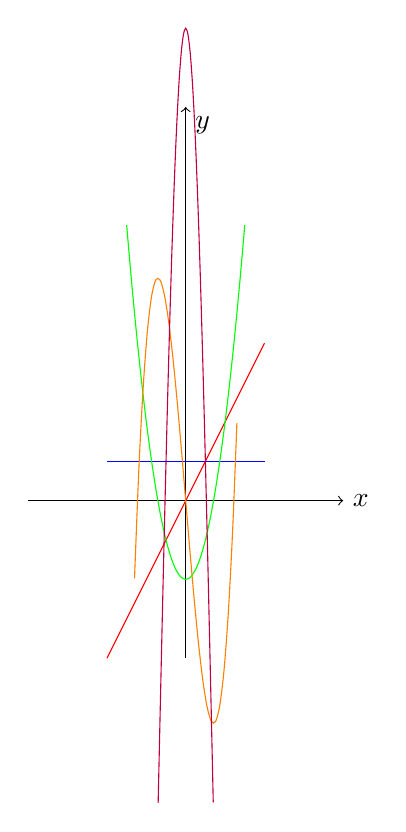
\begin{tikzpicture}
            \draw[->] (-2,0) -- (2,0) node[right] {$x$};
            \draw[->] (0,-2) -- (0,5) node[below right] {$y$};
            \draw[scale=0.5, domain=-2:2, smooth, variable=\x, blue] plot ({\x},{1});
            \draw[scale=0.5, domain=-2:2, smooth, variable=\x, red] plot ({\x},{2*\x});
            \draw[scale=0.5, domain=-1.5:1.5, smooth, variable=\x, green] plot ({\x},{4*(\x)^2-2});
            \draw[scale=0.5, domain=-1.3:1.3, smooth, variable=\x, orange] plot ({\x},{8*(\x)^3-12*\x});
            \draw[scale=0.5, domain=-0.7:0.7, smooth, variable=\x, purple] plot ({\x},{16*(\x)^4-48*(\x)^2+12});
        \end{tikzpicture}
        \caption{Die ersten fünf Hermitepolynome: $H_0$ in blau, $H_1$ in rot, $H_2$ in grün, $H_3$ in orange und $H_4$ in lila.}
    \end{figure}
    Diese Polynome bilden selbst eine Orthonormalbasis des Hilbertraums $L^2(\R)$, sodaß wir jede gegebene Wellenfunktion zerlegen können in die gefundenen Lösungen.
            
\end{document}